\documentclass[tikz]{standalone}
\usetikzlibrary{calc,trees,positioning,arrows,chains,shapes.geometric,%
    decorations.pathreplacing,decorations.pathmorphing,shapes,%
    matrix,shapes.symbols,fit}

\pgfdeclarelayer{back}
\pgfsetlayers{back,main}

\begin{document}
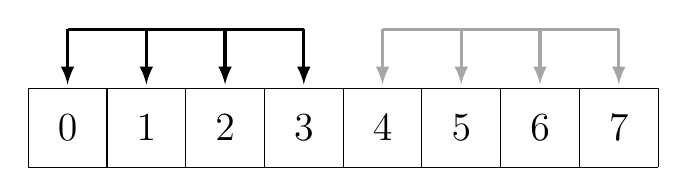
\begin{tikzpicture}
  \draw (0,0) grid (8,1);
  
  \foreach \i in {0,...,7}
  \node[font=\Large{}] at ($(\i,0)+(.5,.5)$) {\i}
  ;
   
  \foreach \i in {0,...,3}
  \draw[very thick,-latex] ($(\i,0)+(.5,1.75)$) -- ($(\i,0)+(.5,1.05)$) 
  ;
  
  \draw[very thick] ($(.5,1.75)$) -- ($(3.5,1.75)$) ;
 
  \foreach \j in {4,...,7}
  \draw[very thick,fill=gray!70,draw=gray!70,-latex] ($(\j,0)+(.5,1.75)$) -- ($(\j,0)+(.5,1.05)$) 
  ;
 
  \draw[very thick,fill=gray!70,draw=gray!70] ($(4.5,1.75)$) -- ($(7.5,1.75)$) ;
\end{tikzpicture}
\end{document}
